\documentclass[../main]{subfiles}

\begin{document}
%%%%%%%%%%%%%%%%%%%%%%%%%%%%%%%%%%%%%%%%%%%%%%%%%%%%%%%%%%%%%%%%%%%%%%%%%
\graphicspath{{images/}}
% To get the right chapter number
\ifSubfilesClassLoaded{
    \externaldocument[main-]{../main}
    \setcounterref{chapter}{main-chap:functies}
    \addtocounter{chapter}{-1}
    \setcounter{page}{\getpagerefnumber{main-chap:functies}}
    % \xsimsetup{
    %     antwoord/print = true% Just for testing purposes
    % }
}{}
%%%%%%%%%%%%%%%%%%%%%%%%%%%%%%%%%%%%%%%%%%%%%%%%%%%%%%%%%%%%%%%%%%%%%%%%%
\renewcommand\lTblrDefaultHruleColorTl{chap_color}

\pagestyle{mypagestyle}
\chapterstyle{MyChapterStyle}  

\chapter{Functies}%
\label{chap:functies}
\begin{objectivesbox}
    \begin{objectiveslist}
        \item ...;
        \item ...;
        \item ....
    \end{objectiveslist}
\end{objectivesbox}

\section{Loops en turtle}%
\label{sec:loops-en-turtle}


%TODO: verwijzen naar eerder hoofdstuk over turtle tekenen
Je hebt inmiddels geleerd hoe je met de turtle module in Python tekeningen kunt maken. Hoe zou je het vierkant in figuur~\ref{fig:turtle-square} kunnen tekenen?

\begin{figure}[h]
    \centering
    \adjustimage{width=6cm}{turtle-square}
    \caption{Vierkant tekenen met turtle}%
    \label{fig:turtle-square}
\end{figure}

Je zou de turtle vier keer vooruit kunnen laten bewegen en telkens 90 graden naar links kunnen laten draaien, zoals in listing~\ref{lst:turtle-vierkant-01}.

\begin{python}[style=mu, caption={Vierkant tekenen met turtle}, label={lst:turtle-vierkant-01}, aboveskip=.5\baselineskip]
import turtle

tony = turtle.Turtle()

tony.fd(100)
tony.lt(90)
tony.fd(100)
tony.lt(90)
tony.fd(100)
tony.lt(90)
tony.fd(100)
tony.lt(90)
\end{python}

De code in listing~\ref{lst:turtle-vierkant-01} werkt prima, maar is eigenlijk niet zo elegant. Je ziet dat in de regels 5 tot en met 12 telkens dezelfde twee instructies worden herhaald. Dat maakt de code langer dan nodig en bovendien lastiger te onderhouden. Als je een groter vierkant zou willen tekenen, bijvoorbeeld met zijden van 200 in plaats van 100, of als je een veelhoek met meer zijden zou willen tekenen, moet je veel regels aanpassen. Door een loop te gebruiken, kun je dit probleem oplossen. In listings~\ref{lst:turtle-vierkant-while} en \ref{lst:turtle-vierkant-for} zie je hoe dat werkt met respectievelijk een \texttt{while} en een \texttt{for} loop.

\noindent\begin{minipage}[t]{.45\textwidth}
\begin{python}[style=mu, caption={Vierkant met while loop}, label={lst:turtle-vierkant-while}]
import turtle

tony = turtle.Turtle()

zijde = 0
while zijde < 4:
    tony.fd(100)
    tony.lt(90)
    zijde += 1
\end{python}
\end{minipage}\hfill
\begin{minipage}[t]{.45\textwidth}
\begin{python}[style=mu, caption={Vierkant met for loop}, label={lst:turtle-vierkant-for}]
import turtle

tony = turtle.Turtle()

for zijde in range(4):
    tony.fd(100)
    tony.lt(90)
\end{python}
\end{minipage}

We zien in beide listings dat de code veel compacter is geworden. Voor de loops wordt een variabele \texttt{zijde} gebruikt die bijhoudt hoeveel zijden van het vierkant al zijn getekend. In de \texttt{while} loop wordt de code herhaald zolang \texttt{zijde} kleiner is dan 4, en in de \texttt{for} loop wordt de code precies 4 keer uitgevoerd. In beide gevallen gaat in elke iteratie de turtle 100 stappen vooruit en draait 90 graden naar links.

\begin{figure}[h]
    \centering
    \adjustimage{width=6cm}{turtle-square-with-sides}
    \caption{Vierkant met een loop}%
    \label{fig:turtle-square-with-sides}
\end{figure}

Met loops kun je niet alleen je code eleganter (en dus beter) maken, maar je tekeningen ook indrukwekkender. Probeer de code in listing~\ref{lst:turtle-meerdere-vierkanten} maar eens uit.

\begin{python}[style=mu, caption={Vierkanten in een loop}, label={lst:turtle-meerdere-vierkanten}, aboveskip=.5\baselineskip]
import turtle

tony = turtle.Turtle()

for vierkant in range(8):
    for zijde in range(4):
        tony.fd(100)
        tony.lt(90)
    tony.lt(45)
    tony.fd(10)
\end{python}

Merk op dat hier sprake is van geneste \texttt{for} loops. De buitenste loop zorgt ervoor dat er 8 vierkanten worden getekend, terwijl de binnenste loop verantwoordelijk is voor het tekenen van één vierkant. Na het tekenen van elk vierkant draait de turtle 45 graden naar links en beweegt 10 stappen vooruit, zodat het volgende vierkant iets gedraaid en verplaatst wordt ten opzichte van het vorige. Regels 9 en 10 zijn even ver ingesprongen als regel 6, wat aangeeft dat ze deel uitmaken van de buitenste loop.

\begin{figure}[h]
    \centering
    \adjustimage{width=6cm}{turtle-multiple-squares}
    \caption{Output van listing~\ref{lst:turtle-meerdere-vierkanten}}%
    \label{fig:turtle-multiple-squares}
\end{figure}

Nóg interessanter wordt het, wanneer je de tellervariabele van de buitenste loop gebruikt om de grootte van de vierkanten aan te passen, zoals in listing~\ref{lst:turtle-meerdere-vierkanten-grootte}.

\begin{python}[style=mu, caption={Vierkanten met toenemende grootte}, label={lst:turtle-meerdere-vierkanten-grootte}, aboveskip=.5\baselineskip]
import turtle

tony = turtle.Turtle()

for vierkant in range(8):
    for zijde in range(4):
        tony.fd(20 + vierkant * 15)
        tony.lt(90)
    tony.lt(45)
    tony.fd(10)
\end{python}

In listing~\ref{lst:turtle-meerdere-vierkanten-grootte} wordt in regel 7 de lengte van elke zijde van het vierkant bepaald door de uitdrukking \texttt{20 + vierkant * 15}. Hierdoor worden de vierkanten steeds groter naarmate de waarde van \texttt{vierkant} toeneemt. Bij de eerste iteratie heeft \texttt{vierkant} de waarde 0, waardoor de zijde 20 stappen lang is. Bij de tweede iteratie is \texttt{vierkant} 1, wat resulteert in een zijde van 35 stappen, enzovoort.

\begin{figure}[h]
    \centering
    \adjustimage{width=6cm}{turtle-growing-squares}
    \caption{Output van listing~\ref{lst:turtle-meerdere-vierkanten-grootte}}%
    \label{fig:turtle-growing-squares}
\end{figure}

\section{Functies en turtle}%
\label{sec:functies-en-turtle}

Wanneer je met turtle tekeningen maakt, zul je merken dat je vaak dezelfde reeks instructies herhaalt. Bijvoorbeeld, in de vorige paragraaf hebben we gezien hoe je een vierkant kunt tekenen met een loop. Maar wat nu als je meerdere vierkanten wilt tekenen op verschillende plaatsen in je tekening? In plaats van telkens dezelfde code opnieuw te typen, kun je beter een functie definiëren die het tekenen van een vierkant verzorgt. Dit maakt je code niet alleen korter, maar ook overzichtelijker en makkelijker te onderhouden.

\begin{python}[style=mu, caption={De functie \texttt{square()}}, label={lst:functie-square-01}, aboveskip=.5\baselineskip]
import turtle

tony = turtle.Turtle()

def square():
    for side in range(4):
        tony.fd(100)
        tony.lt(90)

# HOOFDPROGRAMMA
square()
tony.penup()
tony.fd(150)
tony.pendown()
square()
\end{python}

In listing~\ref{lst:functie-square-01} definiëren we een functie \texttt{square()} die een vierkant tekent met zijden van lengte 100. In het hoofdprogramma roepen we de functie \texttt{square()} twee keer aan, met daartussenin wat code om de turtle te verplaatsen zonder te tekenen.

\begin{figure}[h]
    \centering
    \adjustimage{width=6cm}{turtle-function-square}
    \caption{Output van listing~\ref{lst:functie-square-01}}%
    \label{fig:turtle-two-squares}
\end{figure}

De code in listing~\ref{lst:functie-square-01} heeft een paar nadelen. Ten eerste wordt in de functie \texttt{square()} de \emph{globale} variabele \texttt{tony} gebruikt. Dat heeft tot gevolg dat hij alleen met die specifieke turtle werkt. Wanneer je in je programma meerdere turtles met verschillende namen gebruikt, heb je eigenlijk niets aan deze functie. Daarom is het beter om de turtle als parameter aan de functie door te geven, zodat je dezelfde functie kunt gebruiken met verschillende turtle-objecten. 

\begin{python}[style=mu, caption={De functie \texttt{square(trtl)}}, label={lst:functie-square-02}, aboveskip=.5\baselineskip]
import turtle

tony = turtle.Turtle()
tina = turtle.Turtle()

def square(trtl):
    for side in range(4):
        trtl.fd(100)
        trtl.lt(90)

# HOOFDPROGRAMMA
square(tony)
tina.pencolor('red')
tina.lt(45)
square(tina)
\end{python}

In listing~\ref{lst:functie-square-02} is de functie \texttt{square()} aangepast om een parameter \texttt{trtl} te accepteren, die het turtle-object vertegenwoordigt waarmee het vierkant getekend moet worden. Op regels 8 en 9 gebruiken we nu \texttt{trtl} in plaats van \texttt{tony}.

\begin{figure}[h]
    \centering
    \adjustimage{width=6cm}{turtle-function-square-02}
    \caption{Output van listing~\ref{lst:functie-square-02}}%
    \label{fig:functie-square-02}
\end{figure}

Een tweede nadeel van de functie \texttt{square()} is dat het vierkant altijd zijden van lengte 100 heeft. Je kunt de functie flexibeler maken door een parameter toe te voegen die de lengte van de zijden bevat. Hierdoor kun je vierkanten van verschillende groottes tekenen met dezelfde functie. In listing~\ref{lst:functie-square-03} zie je hoe dat werkt. 

\begin{python}[style=mu, caption={De functie \texttt{square(trtl, size)}}, label={lst:functie-square-03}, aboveskip=.5\baselineskip]
import turtle

tony = turtle.Turtle()

def square(trtl, size = 100):
    for side in range(4):
        trtl.fd(size)
        trtl.lt(90)

# HOOFDPROGRAMMA
square(tony, 50)
tony.penup()
tony.fd(150)
tony.pendown()
square(tony)
\end{python}

In de functiedefinitie is een parameter \texttt{size} toegevoegd, die de lengte van de zijden van het vierkant bepaalt. In het hoofdprogramma roepen we de functie \texttt{square()} twee keer aan: eerst met een argument van 50 en daarna zonder argument, waardoor de standaardwaarde van 100 wordt gebruikt.

\begin{figure}[h]
    \centering
    \adjustimage{width=6cm}{turtle-function-square-03}
    \caption{Output van listing~\ref{lst:functie-square-03}}%
    \label{fig:functie-square-03}
\end{figure}

Telkens wanneer je nu een vierkant wilt tekenen, hoef je slechts de functie \texttt{square()} aan te roepen met de gewenste grootte als argument. Handig hè?

\section{Coördinaten}%
\label{sec:coordinaten}

Tot nu toe bewoog je de turtle met de functies \texttt{turtle.fd()} en \texttt{turtle.bk()} een aantal pixels vooruit of achteruit. En met \texttt{turtle.lt()} en \texttt{turtle.rt()} kon je de turtle naar links of naar rechts laten draaien om vervolgens een andere richting in te slaan. Maar soms is het handiger de turtle in één keer naar een bepaalde plek in het venster te sturen. Bijvoorbeeld naar de hoek linksonder, of naar het middelpunt. Dat kun je doen door coördinaten te gebruiken.

Coördinaten zijn getallen die aangeven waar een punt ligt in een vlak. Wellicht ben je al bekend met geografische coördinaten die we gebruiken om plaatsen op de wereldkaart aan te duiden. Op Google Maps kun je bijvoorbeeld de coördinaten van Gymnasium Beekvliet in Sint-Michielsgestel vinden: (51.642174818007355, 5.3640463837966434).

Om met coördinaten te werken, heb je een assenstelsel nodig. Meestal gebruiken we een horizontale \(x\)-as en een verticale \(y\)-as. In figuur~\ref{fig:coordinatenstelsel} zie je zo'n assenstelsel met drie punten erin uitgezet: (2, 3), (-4, -1) en (5, -2). Het punt (2, 3) ligt bijvoorbeeld 2 eenheden naar rechts op de \(x\)-as en 3 eenheden omhoog op de \(y\)-as. De oorsprong \(O\) is het punt (0, 0), waar de \(x\)-as en \(y\)-as elkaar kruisen.

\begin{figure}[ht]
    \centering
    \scalebox{.8}{
        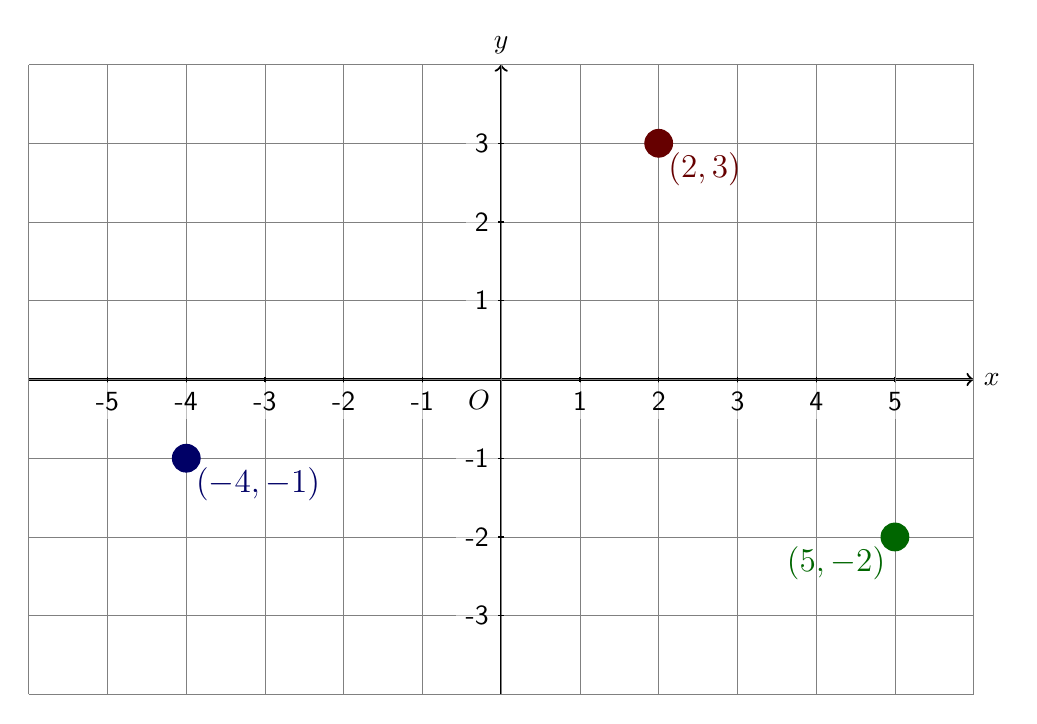
\begin{tikzpicture}[%
            axislabel/.style={%
                font=\sffamily,
                fill=white,
                fill opacity=.5,
                text opacity=1,
            }]
            % Draw axes
            \draw[->, thick] (-6,0) -- (6,0) node[right] {$x$};
            \draw[->, thick] (0,-4) -- (0,4) node[above] {$y$};
            % Draw grid
            \draw[step=1cm,gray,very thin] (-6,-4) grid (6,4);
            % Draw ticks and labels
            \foreach \x in {-5,-4,...,-1,1,2,...,5} {
                \draw (\x,1pt) -- (\x,-1pt) node[below, axislabel] {\x};
            }
            \foreach \y in {-3,-2,-1,1,2,3} {
                \draw(1pt,\y) -- (-1pt,\y) node[left, axislabel] {\y};
            }
            \draw(0,0) node[below left = .5pt] {\(O\)};
            % Plot points
            \filldraw [red!40!black] (2,3) circle (5pt) node[below right, font=\large\bfseries] {\((2,3)\)};
            \filldraw [blue!40!black] (-4,-1) circle (5pt) node[below right, font=\large\bfseries] {\((-4,-1)\)};
            \filldraw [green!40!black] (5,-2) circle (5pt) node[below left, font=\large\bfseries] {\((5,-2)\)};
        \end{tikzpicture}        
    }    
    \caption{Punten met x- en y-coördinaten}
    \label{fig:coordinatenstelsel}
\end{figure}
Zoals je ziet, schrijven we coördinaten altijd als een paar getallen tussen haakjes, waarbij het eerste getal de \(x\)-coördinaat, oftewel de horizontale positie, is en het tweede getal de \(y\)-coördinaat, oftewel de verticale positie.

\subsection*{\texttt{turtle.goto()}}

Met de functie \texttt{turtle.goto(x, y)} kun je de turtle naar specifieke coördinaten sturen.

\begin{minipage}[t]{.45\textwidth}
\begin{python}[style=mu, caption={Vierkant zoals je het al kende}, label={lst:turtle-square-old}, aboveskip=.5\baselineskip]
import turtle

tony = turtle.Turtle()

tony.fd(100)
tony.lt(90)
tony.fd(100)
tony.lt(90)
tony.fd(100)
tony.lt(90)
tony.fd(100)
\end{python}
\end{minipage}\hfill
\begin{minipage}[t]{.45\textwidth}
\begin{python}[style=mu, caption={Vierkant met coördinaten}, label={lst:turtle-square-coordinates}, aboveskip=.5\baselineskip]
import turtle

tony = turtle.Turtle()

tony.goto(100, 0)
tony.goto(100, 100)
tony.goto(0, 100)
tony.goto(0, 0)
\end{python}
\end{minipage}

In het standaard turtle coördinatenstelsel bevindt de oorsprong (0, 0) zich in het midden van het venster en dat is waar de turtle begint. De aanroep \texttt{tony.goto(100, 0)} in regel 5 van listing~\ref{lst:turtle-square-coordinates} verplaatst de turtle 100 stappen naar rechts op de \(x\)-as, terwijl de \(y\)-coördinaat 0 blijft. Vervolgens verplaatst \texttt{tony.goto(100, 100)} de turtle naar het punt (100, 100), wat betekent dat hij niet verder naar rechts, maar wel 100 stappen omhoog gaat. De volgende twee aanroepen verplaatsen de turtle naar (0, 100) en uiteindelijk terug naar (0, 0), waardoor een vierkant wordt getekend (zie figuur~\ref{fig:turtle-square-coordinates}).

\begin{figure}[h]
    \centering
    \adjustimage{width=6cm}{turtle-square-coords}
    \caption{Vierkant met coördinaten}%
    \label{fig:turtle-square-coordinates}
\end{figure}

\subsection*{\texttt{turtle.xcor()} en \texttt{turtle.ycor()}}

Soms wil je de huidige positie van de turtle weten, bijvoorbeeld om berekeningen te maken of om de turtle ergens anders naartoe te verplaatsen op basis van zijn huidige locatie. Hiervoor kun je de functies \texttt{turtle.xcor()} en \texttt{turtle.ycor()} gebruiken, die respectievelijk de huidige \(x\)- en \(y\)-coördinaat van de turtle teruggeven. In listing~\ref{lst:turtle-xcor-ycor} worden deze functies gedemonstreerd door op drie momenten de positie van de turtle af te drukken in de shell.

\begin{python}[style=mu, caption={De coordinaten van de turtle opvragen}, label={lst:turtle-xcor-ycor}, aboveskip=.5\baselineskip]
import turtle

tony = turtle.Turtle()

print(f'Positie 1: ({tony.xcor()}, {tony.ycor()})')
tony.fd(100)
print(f'Positie 2: ({tony.xcor()}, {tony.ycor()})')
tony.lt(90)
tony.fd(100)
print(f'Positie 3: ({tony.xcor()}, {tony.ycor()})')
\end{python}

Bij aanvang van het programma bevindt de turtle zich in de oorsprong, dus de eerste positie is (0.0, 0.0). Na het vooruit bewegen van 100 stappen bevindt de turtle zich op (100.0, 0.0). Vervolgens draait de turtle 90 graden naar links en beweegt weer 100 stappen vooruit, waardoor hij op positie 3 met de coördinaten (100.0, 100.0) terechtkomt (zie figuur~\ref{fig:turtle-xcor-ycor}).

\begin{center}
\shellbox[width=10cm]{turtle\_coords.py}{%
Positie 1: (0.0, 0.0)\\
Positie 2: (100.0, 0.0)\\
Positie 3: (100.0, 100.0)\\
>>>}
\captionof{figure}{Uitvoer van listing \ref{lst:turtle-xcor-ycor}}
\label{fig:turtle-xcor-ycor}
\end{center}

Merk op dat de coördinaten die door \texttt{turtle.xcor()} en \texttt{turtle.ycor()} worden geretourneerd van het type float zijn. Let dus extra goed op het verschil tussen de punten in deze getallen en de komma die we gebruiken om de \(x\)- en \(y\)-coördinaat te scheiden.

%%%%%%%%%%%%%%%%%%%%%%%%%%%%%%%%%%%%%%%%%%%%%%%%%%%%%%%%%%%%%%%%%%%%%
\clearpage
\section*{Opgaven\markright{Opgaven}}

\renewcommand\lTblrDefaultHruleColorTl{black}
%%%%%%%%%%%%%%%%%%%%%%%%%%%%%%%%%%%%%%%%%%%%%%%%%%%%%%%%%%%%%%%%%%%%%
\begin{opgave}[icons={laptop}]
Maak in Mu Editor een nieuw codebestand aan met de naam \file{h\thechapter\_opgave\_\GetExerciseProperty{counter}.py} in de map \folder{Documenten/Pythonprojecten/Oefeningen}. Neem de volgende code over in je bestand:
\begin{python}[style=mu, aboveskip=.5\baselineskip]
import turtle

tony = turtle.Turtle()

zijde = 0
while zijde < 4:
    tony.fd(100)
    tony.lt(90)
    zijde += 1
\end{python}

Deze code tekent een vierkant met behulp van een \texttt{while} loop.

\begin{qlist}
\item Plaats de regels 5 tot en met 9 binnen een tweede \texttt{while} loop die ervoor zorgt dat 3 vierkanten worden getekend. Na het tekenen van elk vierkant moet de turtle naar rechts worden verplaatst zonder te tekenen, zodat de vierkanten naast elkaar komen te staan met een tussenruimte van 50. Om de regels 5 tot en met 9 binnen de buitenste loop te plaatsen, moet je ze inspringen. Dat kun je doen door de regels met de muis te selecteren en vervolgens op \keys{Tab} te drukken.
\begin{center}
    \adjustimage{width=5cm}{turtle-3-squares-2}
\end{center}

\item Pas de buitenste \texttt{while} loop aan zodat er 20 vierkanten worden getekend, niet naast elkaar, maar telkens 18 graden gedraaid ten opzichte van het vorige vierkant. 
\begin{center}
    \adjustimage{width=5cm}{turtle-20-squares-2}
\end{center}

\end{qlist}
\end{opgave}
%--------------------------------------------------------------------
\begin{antwoord}
\begin{qlist}
\item
\begin{python}[style=mu, aboveskip=.5\baselineskip]
import turtle

tony = turtle.Turtle()

vierkant = 0
while vierkant < 3:
    zijde = 0
    while zijde < 4:
        tony.fd(100)
        tony.lt(90)
        zijde += 1
    tony.pu()
    tony.fd(150)
    tony.pd()
    vierkant += 1
\end{python}
\item 
\begin{python}[style=mu, aboveskip=.2\baselineskip]
import turtle

tony = turtle.Turtle()

vierkant = 0
while vierkant < 20:
    zijde = 0
    while zijde < 4:
        tony.fd(100)
        tony.lt(90)
        zijde += 1
    tony.lt(18)
    vierkant += 1
\end{python}
\end{qlist}
\end{antwoord}
%%%%%%%%%%%%%%%%%%%%%%%%%%%%%%%%%%%%%%%%%%%%%%%%%%%%%%%%%%%%%%%%%%%%%
\begin{opgave}[icons={laptop}]
Maak in Mu Editor een nieuw codebestand aan met de naam \file{h\thechapter\_opgave\_\GetExerciseProperty{counter}.py} in de map \folder{Documenten/Pythonprojecten/Oefeningen}. Neem de volgende code over in je bestand:
\begin{python}[style=mu, aboveskip=.5\baselineskip]
import turtle

tony = turtle.Turtle()

def square(trtl, size = 100):
    for side in range(4):
        trtl.fd(size)
        trtl.lt(90)

# HOOFDPROGRAMMA
square(tony)
tony.pu()
tony.fd(150)
tony.pd()
triangle(tony)
\end{python}

\begin{qlist}
\item Op dit moment geeft de code een foutmelding op regel 15, want in het hoofdprogramma wordt de functie \texttt{triangle()} aangeroepen, maar die is nog niet gedefinieerd. Definieer de functie \texttt{triangle()} met een parameter \texttt{trtl} en een parameter \texttt{size} die een standaardwaarde heeft van \texttt{100}. De functie moet een gelijkzijdige driehoek tekenen met zijden van lengte \texttt{size}.
\begin{center}
    \adjustimage{width=6cm}{turtle-function-triangle-2}
\end{center}

\item Vervang de code in het hoofdprogramma door een loop die 5 driehoeken tekent met toenemende grootte, uiteraard door de functie \texttt{triangle()} aan te roepen. De eerste driehoek moet een zijde van 20 hebben, de tweede van 40, de derde van 60, enzovoort. De driehoeken moeten naast elkaar worden getekend, zonder tussenruimte, zoals hieronder wordt getoond:

\begin{center}
    \adjustimage{width=6cm}{turtle-function-triangle-02-2}
\end{center}

\end{qlist}
\end{opgave}
%--------------------------------------------------------------------
\begin{antwoord}
\begin{qlist}
\item
\begin{python}[style=mu, aboveskip=.5\baselineskip]
import turtle

tony = turtle.Turtle()

def square(trtl,size = 100):
    for side in range(4):
        trtl.fd(size)
        trtl.lt(90)
        
def triangle(trtl, size = 100):
    for side in range(3):
        trtl.fd(size)
        trtl.lt(120)
        
# HOOFDPROGRAMMA
square(tony)
tony.pu()
tony.fd(150)
tony.pd()
triangle(tony)
\end{python}
\item Twee mogelijke oplossingen met een \texttt{while} loop:\\
% \begin{minipage}[t]{.4\textwidth}
\begin{python}[style=mu, aboveskip=.2\baselineskip, numbers=none]
# HOOFDPROGRAMMA
n = 1
while n <= 5:
    triangle(tony, 20*n)
    tony.fd(20*n)
    n += 1
\end{python}
% \end{minipage}\hfill

% \begin{minipage}[t]{.5\textwidth}
\begin{python}[style=mu, aboveskip=.2\baselineskip, numbers=none]
# HOOFDPROGRAMMA
n = 20
while n <= 100:
    triangle(tony, n)
    tony.fd(n)
    n += 20
\end{python}
% \end{minipage}\par

Twee mogelijke oplossingen met een \texttt{for} loop:\\
% \begin{minipage}[t]{.4\textwidth}
\begin{python}[style=mu, aboveskip=.2\baselineskip, numbers=none]
# HOOFDPROGRAMMA
for n in range(1, 6):
    triangle(tony, 20*n)
    tony.fd(20*n)
\end{python}
% \end{minipage}\hfill

% \begin{minipage}[t]{.5\textwidth}
\begin{python}[style=mu, aboveskip=.2\baselineskip, numbers=none]
# HOOFDPROGRAMMA
for n in range(20, 120, 20):
    triangle(tony, n)
    tony.fd(n)
\end{python}
% \end{minipage}
\end{qlist}
\end{antwoord}
%%%%%%%%%%%%%%%%%%%%%%%%%%%%%%%%%%%%%%%%%%%%%%%%%%%%%%%%%%%%%%%%%%%%%
\begin{opgave}[icons={laptop}]
\pgfmathparse{int(subtract(\GetExerciseProperty{counter},1))}
Maak in Mu Editor een nieuw codebestand aan met de naam \file{h\thechapter\_opgave\_\GetExerciseProperty{counter}.py} in de map \folder{Documenten/Pythonprojecten/Oefeningen}. Kopieer je code uit \file{h\thechapter\_opgave\_\pgfmathresult.py} naar dit nieuwe bestand. Voeg vervolgens de functie \texttt{filled\_square()} toe zoals hieronder getoond.

\begin{python}[style=mu, aboveskip=.5\baselineskip]
import turtle

tony = turtle.Turtle()

def square(trtl, size = 100):
    for side in range(4):
        trtl.fd(size)
        trtl.lt(90)

def filled_square(trtl, size = 100):
    trtl.begin_fill()
    square(trtl, size)
    trtl.end_fill()

# Overige code weggelaten
\end{python}

Je ziet dat de functie \texttt{filled\_square()} de functie \texttt{square()} aanroept om het vierkant te tekenen. De toevoegingen \texttt{trtl.begin\_fill()} en \texttt{trtl.end\_fill()} zorgen er echter voor dat \texttt{filled\_square()} een gevuld vierkant oplevert.

\begin{qlist}
\item Voeg op dezelfde manier een functie \texttt{filled\_triangle()} toe, die een gevulde driehoek tekent. Wijzig het hoofdprogramma zodat de afbeelding hieronder wordt getekend. Je hebt daarvoor nu slechts twee regels code nodig.
\begin{center}
    \adjustimage{width=2cm}{turtle-function-triangle-03-2}
\end{center}

\item Voeg de functie \texttt{is\_even()} toe waarvan je hieronder de code ziet.

\begin{python}[style=mu, aboveskip=.5\baselineskip, numbers=none]
def is_even(num):
    if num % 2 == 0:
        return True
    return False
\end{python}

Vervang het hoofdprogramma door de volgende code:
\begin{python}[style=mu, aboveskip=.5\baselineskip, numbers=none]
# HOOFDPROGRAMMA
for n in range(8):
    if is_even(n):
        square(tony,40)
    else:
        filled_square(tony, 40)
    tony.fd(40)
\end{python}

Probeer te voorspellen wat het resultaat van deze code zal zijn voordat je het programma uitvoert.

\item Als je begrijpt hoe de code bij vraag b werkt, probeer dan zelf een hoofdprogramma te schrijven dat de onderstaande afbeelding tekent. Dit is een uitdagende vraag; geef het niet te snel op! Je hebt niet per se de functie \texttt{is\_even()} nodig om dit voor elkaar te krijgen.
\begin{center}
    \adjustimage{width=6cm}{turtle-alternating-triangles-2}
\end{center}

\end{qlist}
\end{opgave}
%--------------------------------------------------------------------
\begin{antwoord}
\begin{qlist}
\item De functie \texttt{filled\_triangle()} ziet er als volgt uit:
\begin{python}[style=mu, aboveskip=.5\baselineskip, numbers=none]
def filled_triangle(trtl, size = 100):
    trtl.begin_fill()
    triangle(trtl, size)
    trtl.end_fill()
\end{python}
Het hoofdprogramma is nu:
\begin{python}[style=mu, aboveskip=.5\baselineskip, numbers=none]
# HOOFDPROGRAMMA
square(tony)
filled_triangle(tony)
\end{python}
\item De loop in het hoofdprogramma tekent een rij van 8 vierkanten die afwisselend leeg of gevuld zijn. Voor elke waarde van \texttt{n} wordt gecontroleerd of \texttt{n} even is met behulp van de functie \texttt{is\_even()}. Als \texttt{n} even is, wordt een leeg vierkant getekend; als \texttt{n} oneven is, wordt een gevuld vierkant getekend.

\begin{center}
    \adjustimage{width=6cm}{turtle-alternating-squares}
\end{center}
\item Een mogelijke oplossing voor het hoofdprogramma is:
\begin{python}[style=mu, aboveskip=.5\baselineskip, numbers=none]
# HOOFDPROGRAMMA
for n in range(8):
    if is_even(n):
        triangle(tony,40)
        tony.fd(80)
    else:
        filled_triangle(tony, 40)
    tony.lt(180)
\end{python}
Je zou ook eerst de niet-gevulde driehoeken kunnen tekenen en daarna de gevulde driehoeken. Dan hoef je de \texttt{is\_even()} functie niet te gebruiken. Bijvoorbeeld:
\begin{python}[style=mu, aboveskip=.5\baselineskip, numbers=none]
# HOOFDPROGRAMMA
for n in range(4):
    triangle(tony,40)
    tony.fd(80)
tony.lt(180)
for n in range(4):
    filled_triangle(tony, 40)
    tony.fd(80)
\end{python}
\end{qlist}
\end{antwoord}
%%%%%%%%%%%%%%%%%%%%%%%%%%%%%%%%%%%%%%%%%%%%%%%%%%%%%%%%%%%%%%%%%%%%%
\begin{opgave}[icons={laptop}]
\pgfmathparse{int(subtract(\GetExerciseProperty{counter},1))}
Maak in Mu Editor een nieuw codebestand aan met de naam \file{h\thechapter\_opgave\_\GetExerciseProperty{counter}.py} in de map \folder{Documenten/Pythonprojecten/Oefeningen}. Kopieer je code uit \file{h\thechapter\_opgave\_\pgfmathresult.py} naar dit nieuwe bestand.

In deze opgave gaan we de functies \texttt{square()} en \texttt{filled\_square()} uitbreiden met parameters voor kleur. Wijzig de functie \texttt{square()} als volgt:

\begin{python}[style=mu, aboveskip=.5\baselineskip, numbers=none]
def square(trtl, size = 100, pnclr = 'black'):
    trtl.pencolor(pnclr)
    for side in range(4):
        trtl.fd(size)
        trtl.lt(90)
\end{python}

De functie \texttt{square()} heeft een parameter \texttt{pnclr} gekregen, die de penkleur van de turtle bepaalt. De standaardwaarde is \texttt{'black'}. In de function body wordt de penkleur van de turtle ingesteld met \texttt{trtl.pencolor(pnclr)}.

Gebruik het volgende hoofdprogramma om de aangepaste functie te testen:
\begin{python}[style=mu, aboveskip=.5\baselineskip, numbers=none]
# HOOFDPROGRAMMA
square(tony, 100, 'blue')
triangle(tony)
\end{python}

De uitvoer van het programma ziet er zo uit:
\begin{center}
    \adjustimage{width=2cm}{turtle-function-color-01-2}
\end{center}

Je ziet dat het vierkant nu in het blauw is getekend, maar de driehoek ook! De functie \texttt{square()} heeft de penkleur van de turtle veranderd, en die verandering is ook zichtbaar bij het tekenen van de driehoek. Om dit te voorkomen, moeten we de penkleur na het tekenen van het vierkant weer terugzetten naar de oorspronkelijke kleur.  Dat kan door twee regels code toe te voegen aan het begin en einde van de functie \texttt{square()}:

\begin{python}[style=mu, aboveskip=.5\baselineskip, numbers=none]
def square(trtl, size = 100, pnclr = 'black'):
    old_color = trtl.pencolor()
    trtl.pencolor(pnclr)
    for side in range(4):
        trtl.fd(size)
        trtl.lt(90)
    trtl.pencolor(old_color)
\end{python}

In de eerste regel van de function body slaan we de huidige penkleur op in de variabele \texttt{old\_color}. Na het tekenen van het vierkant zetten we de penkleur weer terug naar de oorspronkelijke kleur met \texttt{trtl.pencolor(old\_color)}. Hierdoor heeft de functie \texttt{square()} geen blijvende invloed meer op de penkleur van de turtle.

Breid nu de functie \texttt{filled\_square()} uit met zowel een parameter voor de penkleur als een parameter voor de vulkleur:

\begin{python}[style=mu, aboveskip=.5\baselineskip, numbers=none]
def filled_square(trtl, size = 100, pnclr = 'black', fllclr = 'black'):
\end{python}

Pas zelf de function body aan en zorg ervoor dat de vulkleur van de turtle na het tekenen weer wordt teruggezet naar de oorspronkelijke waarde.

\pagebreak

Test je code met het volgende hoofdprogramma:
\begin{python}[style=mu, aboveskip=.5\baselineskip, numbers=none]
# HOOFDPROGRAMMA
filled_square(tony, 100, 'red', 'yellow')
triangle(tony)
\end{python}

De uitvoer van het programma ziet er dan zo uit:
\begin{center}
    \adjustimage{width=2cm}{turtle-function-color-02-2}
\end{center}

\end{opgave}
%--------------------------------------------------------------------
\begin{antwoord}

\begin{python}[style=mu, aboveskip=.5\baselineskip, numbers=none]
def filled_square(trtl, size = 100, pnclr = 'black', fllclr = 'black'):
    old_color = trtl.fillcolor()
    trtl.fillcolor(fllclr)
    trtl.begin_fill()
    square(trtl, size, pnclr)
    trtl.end_fill()
    trtl.fillcolor(old_color)
\end{python}

\end{antwoord}
%%%%%%%%%%%%%%%%%%%%%%%%%%%%%%%%%%%%%%%%%%%%%%%%%%%%%%%%%%%%%%%%%%%%%
\begin{opgave}[icons={laptop}]
\pgfmathparse{int(subtract(\GetExerciseProperty{counter},1))}
Maak in Mu Editor een nieuw codebestand aan met de naam \file{h\thechapter\_opgave\_\GetExerciseProperty{counter}.py} in de map \folder{Documenten/Pythonprojecten/Oefeningen}. Kopieer je code uit \file{h\thechapter\_opgave\_\pgfmathresult.py} naar dit nieuwe bestand.

In deze opgave ga je een kunstwerk maken bestaande uit verschillend gekleurde vierkanten die op willekeurige posities worden getekend. Om dat voor elkaar te krijgen, voeg je eerst de functie \texttt{teleport()} toe. Deze functie haalt de pen van het papier, verplaatst de turtle naar een positie en zet de pen weer terug op het papier. De code zie je hieronder.

\begin{python}[style=mu, aboveskip=.5\baselineskip, numbers=none]
def teleport(trtl, x, y):
    trtl.penup()
    trtl.goto(x, y)
    trtl.pendown()
\end{python}

Importeer bovenaan je programma de module \texttt{random} met de regel \texttt{import random}.

\begin{python}[style=mu, aboveskip=.5\baselineskip]
import turtle
import random
\end{python}

\pagebreak

Gebruik het volgende hoofdprogramma om het kunstwerk te maken:
\begin{python}[style=mu, aboveskip=.5\baselineskip, numbers=none]
# HOOFDPROGRAMMA
tony.speed(0)  # Snelste tekensnelheid
colors = ['red', 'yellow', 'blue', 'black']
for n in range(100):
    size = 10 * random.randint(1, 8)
    pen = random.choice(colors)
    fill = random.choice(colors)
    x = random.randint(-300, 300)
    y = random.randint(-200, 200)
    teleport(tony, x, y)
    filled_square(tony, size, pen, fill)
\end{python}

Lijkt jouw kunstwerk op het onderstaande voorbeeld?
\begin{center}
    \adjustimage{width=10cm}{turtle-art}
\end{center}

Gebruik je creativiteit om een origineel kunstwerk te maken. Experimenteer bijvoorbeeld met verschillende kleuren, groottes en aantallen vierkanten. Of gebruik andere vormen zoals driehoeken, rechthoeken (maak je eigen functie \texttt{filled\_rectangle()}) of cirkels. Ook zou je de functie \texttt{square()} kunnen uitbreiden met een parameter voor de pendikte, zodat sommige vierkanten met een dikke pen worden getekend en andere met een dunne pen.

\end{opgave}
%--------------------------------------------------------------------
\begin{antwoord}
*
\end{antwoord}
\clearpage
%%%%%%%%%%%%%%%%%%%%%%%%%%%%%%%%%%%%%%%%%%%%%%%%%%%%%%%%%%%%%%%%%%%%%
\begin{opgave}[icons={laptop}]
\pgfmathparse{int(subtract(\GetExerciseProperty{counter},1))}
Maak in Mu Editor een nieuw codebestand aan met de naam \file{h\thechapter\_opgave\_\GetExerciseProperty{counter}.py} in de map \folder{Documenten/Pythonprojecten/Oefeningen}. Neem de volgende code over in je bestand:

\begin{python}[style=mu, aboveskip=.5\baselineskip]
import turtle

tony = turtle.Turtle()
tony.speed(0)  # Snelste tekensnelheid

def fd_pu(trtl, afstand):
    trtl.penup()
    trtl.fd(afstand)
    trtl.pendown()

def veelhoek(trtl, hoeken, lengte):
    pass

# HOOFDPROGRAMMA
veelhoek(tony, 5, 60)
fd_pu(tony, 100)
veelhoek(tony, 3, 100)
fd_pu(tony, 150)
veelhoek(tony, 8, 36)
\end{python}

Wanneer je deze code uitvoert, gebeurt er niets, omdat de functie \texttt{veelhoek()} nog niet is geïmplementeerd. In regel 12 zie je het keyword \texttt{pass}. Dit betekent dat er nog geen code is, maar dat de functie wel bestaat. Je kunt dit keyword gebruiken als tijdelijke aanduiding wanneer je een functie wilt definiëren, maar nog niet weet wat de inhoud ervan moet zijn. Je mag een functie namelijk niet leeg laten; er moet altijd iets in staan, en \texttt{pass} is daarvoor bedoeld.

Verwijder het \texttt{pass} keyword en programmeer de functie \texttt{veelhoek()} zodat deze een regelmatige veelhoek tekent met het opgegeven aantal hoeken en de opgegeven lengte van de zijden. De uitvoer van het programma zou er ongeveer als volgt uit moeten zien:

\begin{center}
    \adjustimage{width=7cm}{turtle-polygon-2}
\end{center}

\pagebreak

Voor het tekenen heb je een loop nodig, waarbij je twee dingen moet bedenken:
\begin{tasklist}
\item Hoe vaak moet de loop worden uitgevoerd om een veelhoek met het opgegeven aantal hoeken te tekenen?
\item Hoeveel graden moet de turtle na het tekenen van elke zijde draaien?
\end{tasklist}

Vind je het lastig om te berekenen hoeveel graden de turtle telkens moet draaien, kijk dan eens goed naar onderstaande tabel met enkele veelhoeken en hun bijbehorende draaihoeken.

\begin{center}
    \begin{tblr}{
        colspec={Q[l]Q[c]Q[c]Q[c]},
        %column{2-Z} = {font=\ttfamily},
        row{1} = {font=\sffamily\bfseries},
        stretch=1.5}
        \topline
        Vorm & Aantal hoeken & Turtle draaihoek & Totale draaiing \\
        \clinels{1}\clinems{2,3}\cliners{4}
        Driehoek        & 3    & \ang{120}     & 3 \times{} \ang{120} = \ang{360} \\
        Vierkant       & 4    & \ang{90}      & 4 \times{} \ang{90}  = \ang{360}  \\
        Vijfhoek       & 5    & \ang{72}      & 5 \times{} \ang{72}  = \ang{360}  \\
        Zeshoek       & 6    & \ldots{}\si{\degree}      & 6 \times{} \ldots{}\si{\degree}  = \ang{360}  \\
        \bottomline
    \end{tblr}
\end{center}

Hoe zou je de draaihoek voor een zeshoek, zevenhoek of achthoek kunnen berekenen?

\end{opgave}
%--------------------------------------------------------------------
\begin{antwoord}
\begin{python}[style=mu, aboveskip=.5\baselineskip, numbers=none]
def veelhoek(trtl, hoeken, zijde):
    for n in range(hoeken):
        trtl.fd(zijde)
        trtl.lt(360 / hoeken)
\end{python}

Of met een while loop:
\begin{python}[style=mu, aboveskip=.5\baselineskip, numbers=none]
def veelhoek(trtl, hoeken, zijde):
    n = 0
    while n < hoeken:
        trtl.fd(zijde)
        trtl.lt(360 / hoeken)
        n += 1 
\end{python}
\end{antwoord}
%%%%%%%%%%%%%%%%%%%%%%%%%%%%%%%%%%%%%%%%%%%%%%%%%%%%%%%%%%%%%%%%%%%%%
\begin{opgave}[icons={laptop}]
\pgfmathparse{int(subtract(\GetExerciseProperty{counter},2))}
Maak in Mu Editor een nieuw codebestand aan met de naam \file{h\thechapter\_opgave\_\GetExerciseProperty{counter}.py} in de map \folder{Documenten/Pythonprojecten/Oefeningen}.

Definieer een functie die een bloem tekent. Hierbij mag je je eigen creativiteit gebruiken. Maak vervolgens een hoofdprogramma dat meerdere bloemen tekent op verschillende posities in het turtle venster, zodat een bloemenveld ontstaat. Je kunt de functie \texttt{teleport()} uit opgave \pgfmathresult{} gebruiken om de turtle naar verschillende locaties te verplaatsen voordat je een bloem tekent.

\begin{center}
    \adjustimage{width=6cm}{turtle-flowers-2}
\end{center}

\end{opgave}
%--------------------------------------------------------------------
\begin{antwoord}
Het bloemenveld in het voorbeeld is gemaakt met de onderstaande code:
\begin{python-breakable}[style=mu, aboveskip=.5\baselineskip]
import turtle
import random

tony = turtle.Turtle()
tony.screen.bgcolor('dark sea green')
tony.hideturtle()
tony.speed(0)

def flower(trtl, size, petals, petalcolor, centercolor):
    # Bewaar de startpositie voor later
    xstart = trtl.xcor()
    ystart = trtl.ycor()

    # Geef de turtle een willekeurige richting 
    trtl.setheading(random.randint(0, 359))

    # Teken de bloemblaadjes (petals)
    fd_pu(trtl, size * 0.75)
    trtl.lt(90)
    for n in range(petals):
        # Teken eerst een zwarte stip
        trtl.dot(size, 'black')
        # Teken een iets kleinere stip in de petalcolor
        trtl.dot(size - 2, petalcolor)
        # Verplaats een stukje over een cirkelboog
        trtl.pu()
        trtl.circle(size * 0.75, 360 / petals)
        trtl.pd()
    # Verplaats naar de oorspronkelijke positie
    teleport(trtl, xstart, ystart)
    # Teken het hart van de bloem
    trtl.dot(size, centercolor)
    
def teleport(trtl, x, y):
    # Verplaats de turtle zonder te tekenen
    trtl.penup()
    trtl.goto(x, y)
    trtl.pendown()
    
def fd_pu(trtl, afstand):
    # Verplaats de turtle vooruit zonder te tekenen
    trtl.penup()
    trtl.fd(afstand)
    trtl.pendown()
        
# HOOFDPROGRAMMA
petalcolors = ['purple', 'lightblue', 'darkred']
centercolors = ['yellow', 'orange', 'gold']
for n in range(42):
    # Verplaats de turtle naar een willekeurige positie
    x = random.randint(-300, 300)
    y = random.randint(-200, 200)
    teleport(tony, x, y)

    # Teken een bloem met willekeurige eigenschappen
    size = random.randint(20, 50)
    petals = random.randint(5, 7)
    petal = random.choice(petalcolors)
    center = random.choice(centercolors)
    flower(tony, size, petals, petal, center)
\end{python-breakable}
\end{antwoord}
%%%%%%%%%%%%%%%%%%%%%%%%%%%%%%%%%%%%%%%%%%%%%%%%%%%%%%%%%%%%%%%%%%%%%
\section*{Extra oefeningen\markright{Extra oefeningen}}%
\label{sec:extra-oefeningen}

\begin{opgave}[icons={laptop}]
Maak een nieuwe bestand aan in Mu Editor met de naam \file{h\thechapter\_extra\_\GetExerciseProperty{counter}.py}. Schrijf een programma dat onderstaande figuur tekent. De figuur bestaat uit 40 vierkanten. Van binnen naar buiten zijn de zijden van elk vierkant 10 langer dan die van het voorgaande vierkant. De pendikte is 3.

\begin{center}
    \adjustimage{width=6cm}{extra_many_squares}
\end{center}

Je mag voor je programma maximaal 20 regels code gebruiken. Het is niet nodig zelf functies te definiëren om dit probleem te kunnen oplossen, maar het mag natuurlijk wel als je dat wilt.
\end{opgave}
%--------------------------------------------------------------------
\begin{antwoord}
Een mogelijke oplossing:
\begin{python-breakable}[style=mu, aboveskip=.5\baselineskip]
import turtle

tony = turtle.Turtle()
tony.hideturtle()
tony.pensize(3)
tony.speed(0)

for n in range(40):
    for zijde in range(4):
        tony.fd(10 * n)
        tony.lt(90)
    tony.pu()
    tony.bk(5)
    tony.rt(90)
    tony.fd(5)
    tony.lt(90)
    tony.pd()    
\end{python-breakable}
\end{antwoord}
%%%%%%%%%%%%%%%%%%%%%%%%%%%%%%%%%%%%%%%%%%%%%%%%%%%%%%%%%%%%%%%%%%%%%
\begin{opgave}[icons={laptop}]
Maak een nieuwe bestand aan in Mu Editor met de naam \file{h\thechapter\_extra\_\GetExerciseProperty{counter}.py}. Schrijf een programma dat onderstaande figuur tekent. De figuur bestaat uit 15 stippen. De kleinste stip heeft diameter 10 en de grootste stip heeft diameter 80. De ruimte tussen twee opeenvolgende stippen is telkens even groot.

\begin{center}
    \adjustimage{width=0.9\linewidth}{extra_dots}
\end{center}

Je mag voor je programma maximaal 20 regels code gebruiken. Het is niet nodig zelf functies te definiëren om dit probleem te kunnen oplossen, maar het mag natuurlijk wel als je dat wilt.
\end{opgave}
%--------------------------------------------------------------------
\begin{antwoord}
Een mogelijke oplossing:
\begin{python-breakable}[style=mu, aboveskip=.5\baselineskip]
import turtle

tony = turtle.Turtle()
tony.hideturtle()
tony.speed(0)
tony.pu()
tony.bk(300)

for n in range(1, 8):
    tony.dot(10 * n)
    tony.fd(10 * n + 5)
for n in range(8, 0, -1):
    tony.dot(10 * n)
    tony.fd(10 * n - 5)
\end{python-breakable}
\clearpage
Een andere mogelijkheid:
\begin{python-breakable}[style=mu, aboveskip=.5\baselineskip]
import turtle

tony = turtle.Turtle()
tony.hideturtle()
tony.speed(0)
tony.pu()
tony.bk(300)

n = 10
while n <= 70:
    tony.dot(n)
    tony.fd(n + 5)
    n += 10
n = 80
while n >= 10:
    tony.dot(n)
    tony.fd(n - 5)
    n -= 10
\end{python-breakable}
\end{antwoord}
%%%%%%%%%%%%%%%%%%%%%%%%%%%%%%%%%%%%%%%%%%%%%%%%%%%%%%%%%%%%%%%%%%%%%
\clearpage
%%%%%%%%%%%%%%%%%%%%%%%%%%%%%%%%%%%%%%%%%%%%%%%%%%%%%%%%%%%%%%%%%%%%%
\begin{opgave}[icons={laptop}]
Maak een nieuwe bestand aan in Mu Editor met de naam \file{h\thechapter\_extra\_\GetExerciseProperty{counter}.py}. Schrijf een programma waarin de turtle een willekeurige wandeling maakt. Met de functie \texttt{random.randint()} genereer je willekeurige waarden voor:
\begin{itemize}[itemsep=2pt, parsep=0pt, align=left, leftmargin=0.8cm, labelwidth=0.8cm]
\item de \(x\)-coördinaat van de nieuwe positie (tussen -300 en 300)
\item de \(y\)-coördinaat van de nieuwe positie (tussen -200 en 200)
\item de pendikte (tussen 3 en 8)
\end{itemize}
Met behulp van een loop en de functie \texttt{goto()} creëer je vervolgens de willekeurige wandeling van de turtle.

\begin{center}
    \adjustimage{width=0.9\linewidth}{extra_random_walk}
\end{center}

Je mag voor je programma maximaal 20 regels code gebruiken. Het is niet nodig zelf functies te definiëren om dit probleem te kunnen oplossen, maar het mag natuurlijk wel als je dat wilt.
\end{opgave}
%--------------------------------------------------------------------
\begin{antwoord}
Een mogelijke oplossing:
\begin{python}[style=mu, aboveskip=.5\baselineskip]
import turtle, random

tony = turtle.Turtle()
tony.hideturtle()
tony.speed(0)

for n in range(50):
    x = random.randint(-300, 300)
    y = random.randint(-200, 200)
    w = random.randint(3, 8)
    tony.pensize(w)
    tony.goto(x, y)
\end{python}
\end{antwoord}
%%%%%%%%%%%%%%%%%%%%%%%%%%%%%%%%%%%%%%%%%%%%%%%%%%%%%%%%%%%%%%%%%%%%%
\clearpage
%%%%%%%%%%%%%%%%%%%%%%%%%%%%%%%%%%%%%%%%%%%%%%%%%%%%%%%%%%%%%%%%%%%%%
\begin{opgave}[icons={laptop}]
Maak een nieuwe bestand aan in Mu Editor met de naam \file{h\thechapter\_extra\_\GetExerciseProperty{counter}.py}. Neem de onderstaande code over in je bestand.

\begin{python}[style=mu, aboveskip=.5\baselineskip]
import turtle

tony = turtle.Turtle()
tony.hideturtle()
tony.speed(0)

def teleport(trtl, x, y):
    trtl.pu()
    trtl.goto(x, y)
    trtl.pd()

def streepje(trtl, width):
    pass
    
# HOOFDPROGRAMMA
for w in range(1, 15):
    teleport(tony, 0, 20 * w)
    streepje(tony, w)    
\end{python}

Vul de functie \texttt{streepje(trtl, width)} in (verwijder het \texttt{pass} keyword) zodat deze het volgende doet:
\begin{minipage}[t]{.65\textwidth}
\begin{enumerate}[itemsep=2pt, parsep=0pt, align=left, leftmargin=0.8cm, labelwidth=0.8cm]
\item Er wordt een variabele \texttt{length} gedefinieerd die een waarde krijgt gelijk aan 10 keer de breedte (\texttt{width}) van het streepje.
\item De huidige pendikte van de turtle wordt opgeslagen in een variabele \texttt{old\_width}.
\item De pendikte van de turtle wordt veranderd naar de opgegeven breedte (\texttt{width}).
\item Het streepje wordt getekend met de opgegeven lengte (\texttt{length}).
\item De pendikte van de turtle wordt teruggezet naar de oude pendikte (\texttt{old\_width}).
\end{enumerate}
\end{minipage}\hfill
\begin{minipage}[t]{.25\textwidth}
\vspace{.5ex}
\adjustimage{width=\linewidth, valign=t, right}{extra_streepjes}
\end{minipage}\par
\vspace{3\parskip}
Als je het goed hebt gedaan, krijg je 14 (waarom niet 15?) streepjes die naar boven toe steeds dikker en langer worden.
\end{opgave}
%--------------------------------------------------------------------
\begin{antwoord}
\begin{python}[style=mu, aboveskip=.5\baselineskip, numbers=none]
def streepje(trtl, width):
    length = 10 * width
    old_width = trtl.pensize()
    trtl.pensize(width)
    trtl.fd(length)
    trtl.pensize(old_width)
\end{python}
\end{antwoord}
%%%%%%%%%%%%%%%%%%%%%%%%%%%%%%%%%%%%%%%%%%%%%%%%%%%%%%%%%%%%%%%%%%%%%
\clearpage
%%%%%%%%%%%%%%%%%%%%%%%%%%%%%%%%%%%%%%%%%%%%%%%%%%%%%%%%%%%%%%%%%%%%%
\begin{opgave}[icons={laptop}]
Maak een nieuwe bestand aan in Mu Editor met de naam \file{h\thechapter\_extra\_\GetExerciseProperty{counter}.py}. Neem de onderstaande code over in je bestand.

\begin{python}[style=mu, aboveskip=.5\baselineskip]
import turtle, random

tony = turtle.Turtle()
tony.hideturtle()
tony.speed(0)
tony.pensize(3)

def teleport(trtl, x, y):
    trtl.pu()
    trtl.goto(x, y)
    trtl.pd()
    
def square(trtl, x, y, size):
    pass
        
# HOOFDPROGRAMMA
x = random.randint(-300, 300)
y = random.randint(-200, 200)
square(tony, x, y, 100)
teleport(tony, x, y)
tony.dot(100, 'blue')    
\end{python}

Vul de functie \texttt{square(trtl, x, y, size)} in (verwijder het \texttt{pass} keyword) zodat deze een vierkant tekent met de volgende eigenschappen:
\begin{itemize}[itemsep=2pt, parsep=0pt, align=left, leftmargin=0.8cm, labelwidth=0.8cm]
\item Het middelpunt van het vierkant is de positie \((x, y)\).
\item De lengte van de zijden van het vierkant is gelijk aan \texttt{size}.
\end{itemize}
Als je dit goed hebt gedaan, zou de blauwe stip precies in het midden van het vierkant moeten liggen.\par
\adjustimage{width=0.2\linewidth, center, vspace=1ex}{extra_centered_square}
\end{opgave}
%--------------------------------------------------------------------
\begin{antwoord}
Een mogelijke oplossing:
\begin{python}[style=mu, aboveskip=.5\baselineskip, numbers=none]
def square(trtl, x, y, size):
    teleport(trtl, x - size/2, y - size/2)
    for n in range(4):
        trtl.fd(size)
        trtl.lt(90)
\end{python}
\end{antwoord}
%%%%%%%%%%%%%%%%%%%%%%%%%%%%%%%%%%%%%%%%%%%%%%%%%%%%%%%%%%%%%%%%%%%%%
\clearpage
%%%%%%%%%%%%%%%%%%%%%%%%%%%%%%%%%%%%%%%%%%%%%%%%%%%%%%%%%%%%%%%%%%%%%
\begin{opgave}[icons={laptop}]
Maak een nieuwe bestand aan in Mu Editor met de naam \file{h\thechapter\_extra\_\GetExerciseProperty{counter}.py}. Schrijf een programma waarin je een functie definieert die een huisje tekent. Roep in het hoofdprogramma deze functie meerdere keren aan op verschillende posities in het turtle venster, zodat een straat met huisjes ontstaat. Je kunt de functie \texttt{teleport()} uit de vorige opgave gebruiken om de turtle naar verschillende locaties te verplaatsen voordat je een huisje tekent.

Hieronder zie je een voorbeeld, maar voor jouw huisje mag je zelf het ontwerp maken. 

\adjustimage{width=0.7\linewidth, center, vspace=1ex}{extra_houses}
\end{opgave}
%--------------------------------------------------------------------
\begin{antwoord}
*
\end{antwoord}
%%%%%%%%%%%%%%%%%%%%%%%%%%%%%%%%%%%%%%%%%%%%%%%%%%%%%%%%%%%%%%%%%%%%%
\begin{opgave}[icons={laptop}]
Maak een nieuwe bestand aan in Mu Editor met de naam \file{h\thechapter\_extra\_\GetExerciseProperty{counter}.py}.
\begin{qlist}
\item Schrijf een functie \texttt{candle(trtl, length, color)} die een kaars tekent met de opgegeven lengte en kleur.
\item Schrijf een hoofdprogramma dat 7 kaarsen tekent naast elkaar, waarbij de lengte en kleur van elke kaars willekeurig worden gekozen.
\end{qlist}
\adjustimage{width=0.1\linewidth, center, vspace=1ex}{extra_candle}
\end{opgave}
%--------------------------------------------------------------------
\begin{antwoord}
*
\end{antwoord}
%%%%%%%%%%%%%%%%%%%%%%%%%%%%%%%%%%%%%%%%%%%%%%%%%%%%%%%%%%%%%%%%%%%%%

% \clearpage
% \pagestyle{empty}
% \section*{Antwoorden extra opgaven hoofdstuk 12}
% \printsolution[]{opgave}{8}
% \printsolution[]{opgave}{9}
% \printsolution[]{opgave}{10}
% \printsolution[]{opgave}{11}
% \printsolution[]{opgave}{12}
% \printsolution[]{opgave}{13}
% \printsolution[]{opgave}{14}
\end{document}